\documentclass{article}
\usepackage{amssymb, amsmath, amsthm}
\usepackage[margin=1in]{geometry}
\usepackage{verbatim}
\usepackage{graphicx}
\usepackage{hyperref} % \url \href
\usepackage{docmute}
\usepackage{blkarray}

\newtheorem{definition}{Definition}
\newtheorem{theorem}{Theorem}
\DeclareMathOperator{\spn}{Span}

\usepackage[style=chem-acs ,backend=bibtex, sorting=none]{biblatex}
\addbibresource{autoTB.bib}


\begin{document}

\section{Application}
\subsection{Tight-binding band structure cubic Halide Perovskite}

In the work of Boyer et al.\cite{boyer-richard_symmetry-based_2016}, a symmetry adopted 
tightbinding Hamiltonian for cubic Halide Perovskite is constructed. We show that using our 
method, such tightbinding Hamiltonian can be constructed \emph{automatically}. We use the 
crystal structure and atomic coordinates as reported in their work. 

We have in total 16 atomic orbitals in the unit cell, including $s$ and $p$ on Pb and three Cl 
atoms. Pb atoms are octahedral coordinated and three Cl atoms neighbor two Pb atoms along $x$, $y$ 
and $z$ direction. We use the same neighbors as used in their work. Free parameter extraction 
produce the results listed in Table \ref{T:free_perovskite}.

\begin{table}[h!]
    \centering
    \caption{Free Interaction Parameters Extracted Using Our Methods for Cubic Halide Perovskite}
    \begin{tabular}{|l|c|c|}
        \hline
        sites & position & interactions \\
        \hline
        Pb & $(0.0,0.0,0.0)$ & $\langle \chi_s^{Pb} | H | \chi_s^{Pb} \rangle$, $\langle \chi_{p_x}^{Pb} | H | \chi_{p_x}^{Pb} \rangle$ \\
        \hline
        Cl & $(0.5,0.0,0.0)$ & $\langle \chi_s^{Cl} | H | \chi_s^{Cl} \rangle$, $\langle \chi_{p_x}^{Cl} | H | \chi_{p_x}^{Cl} \rangle $, $\langle \chi_{p_z}^{Cl} | H | \chi_{p_z}^{Cl} \rangle$ \\
        \hline
        Interaction & & $\langle \chi_s^{Pb} | H | \chi_s^{Cl} \rangle$, $\langle \chi_{p_x}^{Pb} | H | \chi_s^{Cl} \rangle$, $\langle \chi_s^{Pb} | H | \chi_{p_x}^{Cl} \rangle$, 
        $\langle \chi_{p_x}^{Pb} | H | \chi_{p_x}^{Cl} \rangle$, $\langle \chi_{p_z}^{Pb} | H | \chi_{p_z}^{Cl} \rangle$ \\
        \hline
    \end{tabular}
    \label{T:free_perovskite}
\end{table}

All the free interactions are found by our method. Furthermore, it is interesting to note that one additional parameters are obtained,
as compared to the original work. For Cl atom, two of its $p$ function are degenerate in energy while the third $p$ function along the 
$Pb$ direction should have a different energy. This is missed by the work of Boyer et al. but is discovered 
systematically by our methods.
Assigning the reported values to these interactions and construct tightbinding model, we obtain the band structure, comparable to reported 
by Boyer et al, as shown in Figure \ref{F:Application_Perovskite_band}. We note that in our implementation, SOC is not taken account. 
The whole process, from analysize the structure to solving the band structure, took within a few seconds.

\begin{figure}[h!]
    \centering
    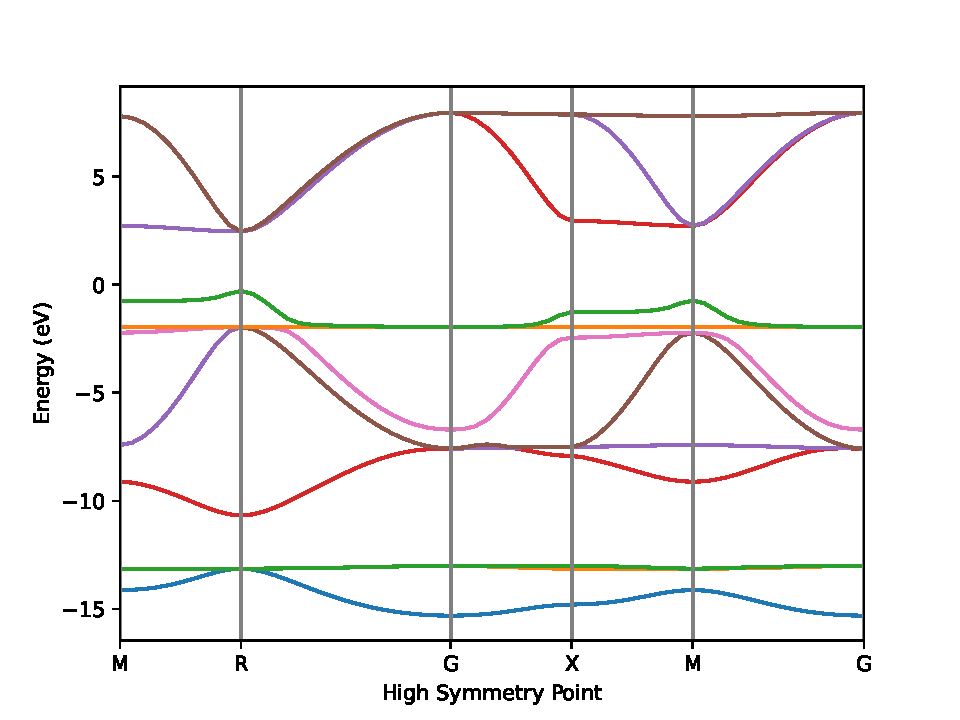
\includegraphics[width=3in]{../figures/HalidePerovskite_band.pdf}
    \caption{Bandstructure obtained from constructed tight binding model for cubic Halide Perovskite}
    \label{F:Application_Perovskite_band}
\end{figure}


\end{document}